\documentclass{amsart}
\usepackage{graphicx}
\usepackage[RGB]{xcolor}
\usepackage{tikz}

% \colorsquare{#1: color}{#2 x-coordinate}{#3: y-coordinate}
% the bottom left coordinate is (1,1), and the topright of an nxn square is (n,n)
\newcommand{\colorsquare}[3]{
\coordinate (pos) at (#2-1,#3-1);
\filldraw[color=#1] (pos)--++(1,0)--++(0,1)--++(-1,0)--cycle;
}

% \numbersquare{#1: int}{#2: x-coordinate}{#3: y-coordinate}
% uses the same coordinate scheme as \colorsquare
\newcommand{\numbersquare}[3]{\draw(#2-.5, #3-.5) node {\LARGE $\mathsf{#1}$};}

\newcommand{\drawthick}{\draw[line width=1.75pt]}

\definecolor{I}{RGB}{238,170,169}
\definecolor{F}{RGB}{220,187,153}
\definecolor{L}{RGB}{204,204,136}
\definecolor{P}{RGB}{186,221,153}
\definecolor{N}{RGB}{169,238,170}
\definecolor{T}{RGB}{153,221,187}
\definecolor{U}{RGB}{136,204,204}
\definecolor{V}{RGB}{153,187,221}
\definecolor{W}{RGB}{170,170,238}
\definecolor{X}{RGB}{186,153,221}
\definecolor{Y}{RGB}{204,136,204}
\definecolor{Z}{RGB}{221,153,186}

% \drawgrid{#1: int}
% draws an #1x#1 grid with thick lines around the border
\newcommand{\drawgriddotted}[1]{
    \foreach \x in {0,...,#1}{
    \draw[densely dotted] (\x,#1)--(\x,0);
    }
    \foreach \y in {0,...,#1}{
      \draw[densely dotted] (0,\y)--(#1,\y);
    }
   \drawthick (0,0)--(0,#1)--(#1,#1)--(#1,0)--cycle;
}

\newcommand{\drawgridthin}[1]{
    \foreach \x in {0,...,#1}{
    \draw[very thin] (\x,#1)--(\x,0);
    }
    \foreach \y in {0,...,#1}{
      \draw[very thin] (0,\y)--(#1,\y);
    }
   \drawthick (0,0)--(0,#1)--(#1,#1)--(#1,0)--cycle;
}
    
\begin{document}
\resizebox{30pc}{!}{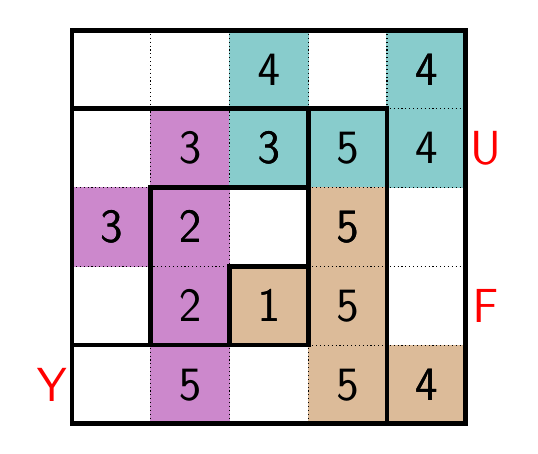
\begin{tikzpicture}
\colorsquare{Y}{2}{1}\colorsquare{Y}{1}{3}\colorsquare{Y}{2}{4}\colorsquare{Y}{2}{2}\colorsquare{Y}{2}{3}
\colorsquare{U}{4}{4}\colorsquare{U}{3}{4}\colorsquare{U}{5}{5}\colorsquare{U}{3}{5}\colorsquare{U}{5}{4}
\colorsquare{F}{4}{1}\colorsquare{F}{3}{2}\colorsquare{F}{4}{2}\colorsquare{F}{4}{3}\colorsquare{F}{5}{1}
\drawthick (4,4)--++(-4,0)--++(0,1)--++(5,0)--++(0,-5)--++(-1,0)--cycle;
    \drawthick (3,0)--++(-3,0)--++(0,1)--++(3,0)--++(0,3)--++(1,0)--++(0,-4)--cycle;
    \drawthick (0,3)--++(0,1)--++(3,0)--++(0,-1)--++(-2,0)--++(0,-2)--++(-1,0)--cycle;
    \drawthick (1,2)--++(0,1)--++(2,0)--++(0,-1)--++(-1,0)--++(0,-1)--++(-1,0)--cycle;\drawgriddotted{5}\numbersquare{3}{1}{3}\numbersquare{2}{2}{3}\numbersquare{1}{3}{2}\numbersquare{3}{3}{4}\numbersquare{5}{4}{3}\numbersquare{4}{5}{1}\numbersquare{4}{5}{5}\numbersquare{\textcolor{red}{U}}{5.75}{4.0}\numbersquare{\textcolor{red}{Y}}{0.25}{1.0}\numbersquare{\textcolor{red}{F}}{5.75}{2.0}\numbersquare{5}{2}{1}\numbersquare{3}{1}{3}\numbersquare{3}{2}{4}\numbersquare{2}{2}{2}\numbersquare{2}{2}{3}\numbersquare{5}{4}{4}\numbersquare{3}{3}{4}\numbersquare{4}{5}{5}\numbersquare{4}{3}{5}\numbersquare{4}{5}{4}\numbersquare{5}{4}{1}\numbersquare{1}{3}{2}\numbersquare{5}{4}{2}\numbersquare{5}{4}{3}\numbersquare{4}{5}{1}\end{tikzpicture}}
\vspace{1pc}

\noindent\Large{\tt The product of the areas of the connected unfilled squares is 12}
\end{document}